\documentclass[tikz,border=10pt]{standalone}
\begin{document}
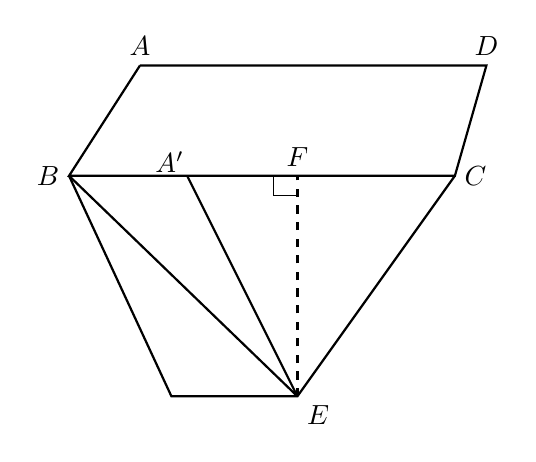
\begin{tikzpicture}
\coordinate (A) at (1.2,4.2);
\coordinate (D) at (5.6,4.2);
\coordinate (B) at (0.3,2.8);
\coordinate (C) at (5.2,2.8);
\coordinate (A1) at (1.8,2.8);
\coordinate (F) at (3.2,2.8);
\coordinate (E) at (3.2,0);
\coordinate (G) at (1.6,0);

\draw[thick] (A) -- (D) -- (C) -- (B) -- (A);
\draw[thick] (B) -- (C);
\draw[thick] (B) -- (G) -- (E) -- (C);
\draw[thick] (A1) -- (E);
\draw[thick] (B) -- (E);
\draw[dashed,thick] (E) -- (F);
\draw (2.9,2.8) -- (2.9,2.55) -- (3.2,2.55);

\node[above] at (A) {$A$};
\node[above] at (D) {$D$};
\node[left] at (B) {$B$};
\node[right] at (C) {$C$};
\node[above left,inner sep=1pt] at (A1) {$A'$};
\node[above] at (F) {$F$};
\node[below right] at (E) {$E$};
\end{tikzpicture}
\end{document}
